% !TEX root = ../main.tex
\section{Critical Evaluation and Limitations}

\subsection{Trend in the data source}

The raw crawl shows a sharp decline (Figure~\ref{fig:trend}). Monthly questions on Stack Overflow fell by
98\%, from 47,570 in January 2024 to 843 in October 2026, and AI/ML questions fell at the same rate (2,071
to 30), staying at about 4.5\% of the total. The share of AI/ML questions that received an answer stayed
near 71\% until mid-2026, dropping only in the last months, which have had less time to be answered. The
fall is therefore in questions being asked, not in answers. A likely cause is the move to LLM
assistants, though our data cannot prove it.

For StackLearn, this means coverage of new libraries will grow slowly, since 75\% of the catalog dates
from 2024, and collecting more data later will add little. The product's value lies in making this
existing, community-checked knowledge easy to find, alongside LLM answers that nobody has verified.

\begin{figure}[h]
  \centering
  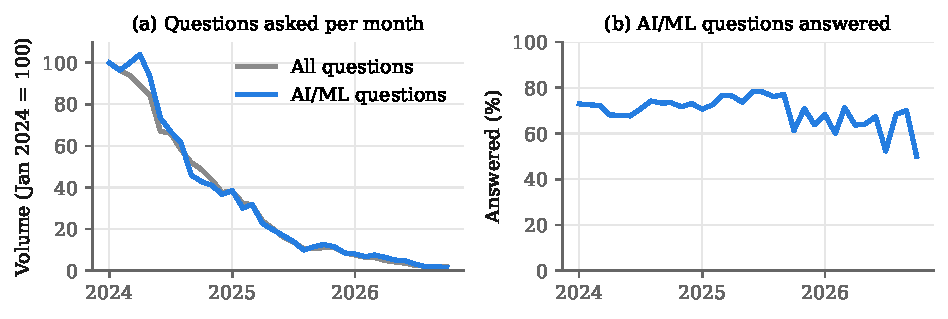
\includegraphics[width=0.9\linewidth]{figures/trend.pdf}
  \caption{Raw crawl, January 2024 to October 2026. (a) Monthly questions, indexed to January 2024 = 100;
  (b) share of AI/ML questions with at least one answer.}
  \label{fig:trend}
\end{figure}

\subsection{Limitations}

Our relevance measure is generous: two \texttt{pytorch} questions can be about unrelated problems, so
absolute P@k values overstate usefulness, although the model comparison stays fair. The 16,861 duplicate
links we collected would allow a stricter test. The random split
also lets a query be older than its matches; a split by date would be more realistic. Finally, MiniLM
could be fine-tuned on the duplicate pairs, and the \texttt{keras} result suggests combining word
matching with embeddings for queries containing exact class names.
